\chapter{Das Tor ins Nichts}
\noindent\textbf{Akt II, Szene 5:} Die vier Wächter, die andere Welt und die Flucht\\
\textbf{Ziel:} Flynn retten, den sehenden Stein in die Fassung der schwebenden Plattform einsetzen, den Übergang schlie\ss{}en und die zerfallende Anlage verlassen.

\begin{meisterinfo}
\textbf{Die Wahrheit:} Dr. Skorbinsk hielt das Auge für einen Schlüssel zur Öffnung. Tatsächlich dient der Stein als Siegel einer uralten Grenzvorrichtung. Seine Entnahme lie\ss{} den Durchgang instabil werden; die vier Statuen begrenzen ihn. Zeitliche Echos erklären die Karte in Arkham, die Erscheinung Yusufs und die anomalen Zustände im Carlson-Haus. Die genauen Gesetze bleiben auch nach dem Finale unbegreiflich. \textbf{Flynn} lebt auf der Plattform und ist rettbar. \textbf{Skorbinsk} starb in der Statuenhalle. \textbf{Der Stein bleibt nach dem Verschlie\ss{}en endgültig in der Plattform zurück und geht mit der anderen Dimension verloren. Er wird nicht wiedergefunden und verwandelt sich nicht in ein Älteres Zeichen.} Die Abbildungen zeigen Spielleitungsillustrationen, keine zwingend wortwörtliche Architektur.
\end{meisterinfo}

\section{5.1 -- Die Halle der vier Wächter}
\begin{vorlesetextalle}
Ihr tretet durch den dunklen Durchgang in eine Halle von gewaltigen Ausma\ss{}en. Vier hohe steinerne Gestalten stehen um eine kreisförmige Bodenfläche; ihre glatten Gesichter und langen Stäbe wirken weder ägyptisch noch menschlich vertraut. Ihre Blicke richten sich über die Mitte hinweg auf ein riesiges, weit geöffnetes Tor. Dahinter ist keine Mauer, kein weiterer Raum, sondern eine Dunkelheit mit fernen, unsteten Lichtpunkten. Eure Lampen vermögen ihre Tiefe nicht zu ergründen.
\end{vorlesetextalle}
\begin{meisterinfo}
\textbf{Archäologie:} Die Statuen sind älter als die ägyptisch anmutenden Ergänzungen. \textbf{Verborgenes Erkennen:} Linien unter ihren Sockeln laufen auf das Tor zu. \textbf{Okkultismus:} Die vier Wächter begrenzen einen Übergang, statt selbst anzugreifen. \textbf{Idee:} Skorbinsks Skizze mit vier Markierungen zeigt genau diese Anordnung. Das Tor ist bereits geöffnet; es braucht kein zusätzliches Öffnungsritual. \textbf{Fundabsicherung:} Falls der sehende Stein zuvor nicht aufgenommen wurde, liegt er deutlich sichtbar unmittelbar vor der Schwelle. Er kann ohne Probe genommen werden.
\end{meisterinfo}

\section{5.2 -- Dr. Skorbinsks letztes Zeugnis}
\begin{vorlesetextalle}
Am Sockel einer Statue sitzt ein regloser Mann. Kleidung und Gesicht sind von Staub bedeckt; neben seiner Hand liegen verstreute Blätter und eine zerbrochene Brille. Ihr erkennt Dr. Skorbinsk. Seine Augen starren unverwandt auf das offene Tor. Auf einem der Blätter stehen hastig geschriebene Worte: \glqq{}Ich dachte, es sei ein Schlüssel. Ich verstand nicht, dass es ein Siegel war. Vier halten die Grenze. Das Auge schlie\ss{}t.\grqq{}
\end{vorlesetextalle}
\begin{meisterinfo}
\textbf{Medizin:} Skorbinsk ist tot, ohne klare äu\ss{}ere Todesursache. \textbf{Stabilität:} 0/1W3 STA beim Auffinden. \textbf{Folgerung:} Stein und vier Wächter gehören zusammen; der Abschluss findet jenseits des Tores statt. Skorbinsk ist nicht als Kampfgegner vorgesehen.
\end{meisterinfo}

\section{5.3 -- Blick durch das Tor}
\begin{figure}[htbp]\centering
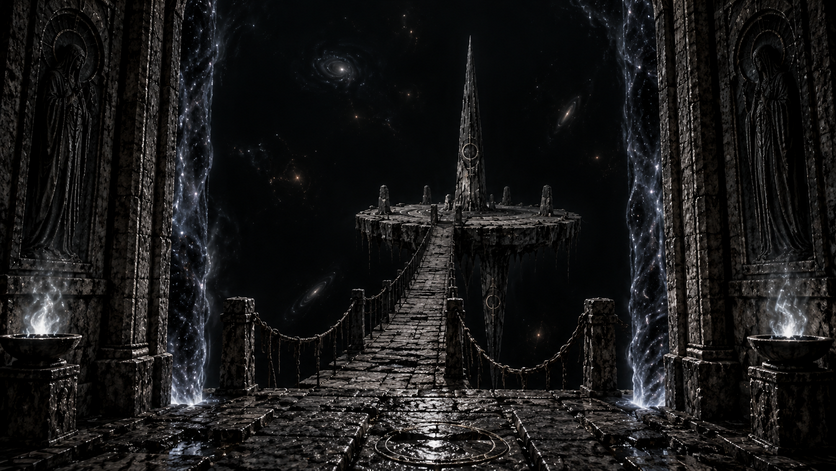
\includegraphics[width=\textwidth]{bilder/finale-tor-im-nichts.png}
\caption{Blick von der steinernen Schwelle zur frei schwebenden Plattform im Nichts.}
\end{figure}
\begin{vorlesetextalle}
Durch das Tor führt eine schmale Hängebrücke aus dunklen Steinplatten, gehalten von schweren Ketten. Sie endet an einer etwa fünf Meter breiten, kreisrunden Plattform, die frei in einer endlosen Dunkelheit schwebt. Aus ihrer Mitte erhebt sich eine steinerne Nadel; eine zweite, ebenso spitze ragt von ihrer Unterseite hinab. Weit entfernt funkeln Lichtpunkte wie Sterne, doch sobald Ihr sie fixiert, scheinen sich ihre Entfernungen zu verändern. Kein Horizont, kein Oben, kein Unten gibt Euch Halt. Ein bedrückendes Gefühl breitet sich in Eurer Brust aus, als wäre die Unendlichkeit selbst zu schwer für Eure Gedanken.
\end{vorlesetextalle}
\begin{meisterinfo}
\textbf{Stabilität:} Beim ersten ungeschützten Blick 1/1W6 STA. \textbf{Schwelle:} Der Atem ist möglich; die Luft folgt hier offenbar eigenen Regeln. Die Brücke ist begehbar und trägt die Gruppe, auch wenn sie schwankt. \textbf{Orientierung oder Idee:} Wer sich auf einzelne Schritte statt auf die Ferne konzentriert, kann ruhiger vorankommen.
\end{meisterinfo}

\section{5.4 -- Die Brücke und ihre Rückseite}
\begin{vorlesetextalle}
Die Platten schwingen leicht unter Euren Schuhen. Je weiter Ihr geht, desto unwirklicher wird die Entfernung zur Plattform. Als Ihr zurückblickt, erkennt Ihr die Rückseite des steinernen Tores frei im Nichts. Die Statuenhalle ist von hier aus verschwunden; allein der Rahmen hängt ohne Stütze in der grenzenlosen Leere. Für einen schrecklichen Moment fragt Ihr Euch, ob jenseits der Schwelle überhaupt noch Eure Welt existiert.
\end{vorlesetextalle}
\begin{meisterinfo}
\textbf{Stabilität:} Beim erstmaligen Erkennen der frei schwebenden Rückseite 0/1W3 STA. Nach jeweils weiteren fünf Minuten auf Brücke oder Plattform 0/1W3 STA; nicht in jeder Runde wiederholen. \textbf{Interaktion:} Orientierung (Rhythmus der Schritte), Psychologie (Gefährten beruhigen), Klettern und Stärke (Hilfe bei einem Stolpern). Fehlwürfe kosten Zeit oder verursachen eine brenzlige Lage, nicht automatisch einen Absturz. \textbf{Rückweg:} Trotz optischer Verwirrung bleibt der Übergang erreichbar.
\end{meisterinfo}

\section{5.5 -- Flynn Carlson auf der Plattform}
\begin{vorlesetextalle}
Die Plattform besteht aus ebenem schwarzem Stein, in den konzentrische Linien eingearbeitet wurden. Zwischen ihnen befindet sich eine handtellergro\ss{}e Vertiefung mit dem Zeichen des Auges. Am Fu\ss{} der aufragenden Nadel kauert ein erschöpfter Mann in zerrissener Kleidung. Er hebt langsam den Kopf. \glqq{}Seid Ihr wirklich hier? Oder seid Ihr wieder eine Erscheinung?\grqq{} Seine Stimme ist kaum mehr als ein Flüstern. \glqq{}Ich bin Flynn Carlson. Wie lange bin ich hier?\grqq{}
\end{vorlesetextalle}
\begin{meisterinfo}
\textbf{Flynn lebt:} Für ihn könnten subjektiv nur Tage vergangen sein. \textbf{Erste Hilfe/Medizin:} Schwäche, Durst und Desorientierung; er ist gestützt transportfähig. \textbf{Psychologie:} Ruhiges Ansprechen hilft ihm, bei der Gruppe zu bleiben. Er kann berichten, dass Skorbinsk das Artefakt als Schlüssel verstand und dass nach dem Öffnen fremde Wesen erschienen. Von Helenas Tod wei\ss{} er nichts; ob die Ermittler ihn hier darüber informieren, entscheiden die Spieler. \textbf{Sicherheit:} Er darf gerettet werden, ohne dass ein Einzelwurf das Schicksal automatisch festlegt.
\end{meisterinfo}

\section{5.6 -- Das Siegel wird eingesetzt}
\begin{vorlesetextalle}
Als Ihr den Stein mit dem Auge über die Vertiefung hebt, beginnt seine Gravur fahl zu leuchten. Das Artefakt gleitet in die Fassung und sitzt darin vollkommen fest. Silberne Linien breiten sich über den Boden aus; die beiden Steinnadeln beginnen zu vibrieren. Um Euch ziehen sich ferne Lichtpunkte zusammen. Dann hört Ihr eine Stimme, die von keinem bestimmten Ort zu kommen scheint: \glqq{}Endlich.\grqq{}
\end{vorlesetextalle}
\begin{meisterinfo}
\textbf{Keine Probe notwendig:} Das Einsetzen ist die Lösung. Eine gelungene Idee- oder Okkultismusprobe darf zuvor einen Hinweis geben. \textbf{Unwiderruflich:} Der Stein verschmilzt mit der Fassung und ist nicht mehr herauszulösen. Er bleibt in der sich auflösenden jenseitigen Konstruktion und ist endgültig verloren. Mit dem Einsetzen beginnt der Verschluss, zugleich aber der Zerfall der Anlage. \textbf{Nicht den Sieg durch eine weitere Pflichtprobe entwerten.}
\end{meisterinfo}

\section{5.7 -- Bast, die Hüterin der Grenze}
\begin{vorlesetextalle}
Vor Euch flimmert die Dunkelheit. Eine schlanke Gestalt tritt hervor, von beinahe menschlicher Haltung, doch mit dem Haupt und den Augen einer Katze. Ein schlichtes Gewand umhüllt ihren Körper. Sie betrachtet die leuchtende Fassung. \glqq{}Die Grenze wird wiederhergestellt. Ihr habt geschlossen, was nicht hätte offen stehen dürfen. Durch diese Schwelle kamen Dinge in Eure Welt, die dort keinen Platz haben. Wäre sie geblieben, wären andere gefolgt.\grqq{} Ein gewaltiges Grollen erschüttert die Plattform. \glqq{}Die Verbindung zerfällt nun, und mit ihr die Steine, die sie halten. Geht. Nehmt den Lebenden mit. Kehrt zurück, ehe der Weg vergeht.\grqq{} Ihre Augen verweilen einen letzten Moment auf Euch. \glqq{}Nicht alles, was Euch sieht, wünscht Euch Schaden.\grqq{} Dann verblasst ihre Erscheinung.
\end{vorlesetextalle}
\begin{meisterinfo}
\textbf{Bast ist keine Gegnerin.} Sie erläutert nur das unbedingt Nötige: Tor offen, fremde Wesen (darunter der Dhole), Gefahr für die Welt, jetzt Verschluss und Kollaps. Die Vision soll kurz bleiben. Kein zusätzlicher Stabilitätswurf nötig. \textbf{Stein:} Bast gibt ihn nicht zurück und verspricht auch keinen Ersatz.
\end{meisterinfo}

\section{5.8 -- Rückweg über die brechende Brücke}
\begin{vorlesetextalle}
Ein Krachen läuft durch die Nadel. Die Plattform schwankt und ein Stück Fels bricht an ihrem Rand ab, ohne irgendwo aufzuschlagen. Die Ketten der Brücke spannen sich knarrend. Am fernen Ende scheint das Tor mal die Statuenhalle, mal nur eine dunkle Oberfläche zu zeigen. Ein weiterer Ruck zwingt Euch, Halt zu suchen. Ihr müsst zurück -- und Flynn kann kaum allein gehen.
\end{vorlesetextalle}
\begin{meisterinfo}
\textbf{Drei Phasen:} (1) Flynn aufrichten und die Plattform verlassen (Stärke, Erste Hilfe, Teamarbeit); (2) über die schwankende Brücke (Klettern, Springen, Verborgenes Erkennen, Seilsicherung); (3) geschlossen durch das Tor gelangen (Orientierung, Absprachen, Rettungsversuche). Erfolgreiche clevere Ideen zählen wie Proben. Fehlschläge kosten Zeit, Ausrüstung oder verursachen kleinere Verletzungen. Eine tödliche Konsequenz nur nach deutlich angekündigten Risiken und mehrfachen Fehlschlägen. Die Erkundung soll nicht mit einer zufälligen Einzelprobe enden.
\end{meisterinfo}

\section{5.9 -- Das Tor wird zu nacktem Stein}
\begin{vorlesetextalle}
Ihr stolpert durch die Schwelle zurück auf festen Boden. Hinter Euch hängt die Brücke noch im Nichts, doch ihre Konturen werden blass. Die Sterne verlöschen, die Plattform und ihre Nadeln zerflie\ss{}en im Dunkel. Wo eben noch unendlicher Raum lag, wird eine kahle Felswand sichtbar. Schlie\ss{}lich steht das Tor vor nichts anderem als festem Stein. Dann splittert eine der vier Statuen. Das Krachen weiterer Risse erfüllt die Halle. Gewaltige Blöcke stürzen zu Boden.
\end{vorlesetextalle}
\begin{meisterinfo}
Die vier Statuen waren Grenzwächter, keine Kampfgegner. Mit dem geschlossenen Übergang verlieren sie ihre Funktion und zerfallen. Das Tor bleibt auf dieser Seite nur ein bedeutungsloser Rahmen vor einer Felswand. Der Stein ist nicht hier, sondern im verlorenen Jenseits.
\end{meisterinfo}

\section{5.10 -- Flucht aus den zerfallenden Katakomben}
\begin{vorlesetextalle}
Die Halle bebt. Staub und Steinsplitter regnen von der Decke. Ihr eilt durch bekannte Gänge, doch an mehreren Stellen versperren herabgestürzte Blöcke den Weg. Hinter Euch donnert ein tiefer Einsturz durch die Anlage. Aus der Ferne klingt das Brechen schwerer Gesteinsmassen wie ein Gewitter unter der Erde. Vor Euch liegt irgendwo der Ausgang zur Wüste.
\end{vorlesetextalle}
\begin{meisterinfo}
\textbf{Gruppenherausforderung:} Fünf Erfolge vor drei schweren Rückschlägen. Jede Figur beschreibt einen sinnvollen Beitrag; nicht immer denselben Wurf wiederholen. Geeignet: Orientierung mit Flynns Karte, Stärke zum Freiräumen, Klettern/Springen, Verborgenes Erkennen für instabile Decken, Erste Hilfe für Verletzte, Psychologie gegen Panik. Erfolge schaffen echte Fortschritte. Fehlschläge führen zu verlorener Zeit, verlorener Ausrüstung oder einer Verletzung. Bei drei Rückschlägen folgt ein letzter schwieriger Ausgang statt automatischer Gruppenvernichtung. Flynn braucht Hilfe, darf aber bei kluger Zusammenarbeit mitgerettet werden.
\end{meisterinfo}

\section{5.11 -- Wieder unter der Sonne}
\begin{vorlesetextalle}
Endlich erscheint Tageslicht. Ihr stolpert aus der Felsöffnung in warme, trockene Luft. Hinter Euch knicken hölzerne Stützen ein, ein tiefes Donnern läuft durch den Berghang. Geröll stürzt herab und verschüttet den Eingang vollständig. Dann legt sich der Staub. Wo die Expedition einst die unterirdische Anlage freigelegt hatte, liegt nur noch gewöhnlicher Stein. Über Euch spannt sich ein blauer Himmel. Zum ersten Mal seit Langem fühlt sich die Welt wieder vertraut an.
\end{vorlesetextalle}

\chapter*{Epilog -- Was bleibt}
\addcontentsline{toc}{chapter}{Epilog -- Was bleibt}
\begin{vorlesetextalle}
Die Tage nach Eurer Flucht sind erfüllt von Rückreisevorbereitungen, Erschöpfung und Gesprächen über das Unbegreifliche. Flynn Carlson hat die Katastrophe überlebt. Doch die Nachricht vom Tod seiner Frau liegt schwer auf ihm, und seine Erinnerungen an die schwebende Plattform folgen ihm bis in den Schlaf. Als Ihr Arkham wieder erreicht, bleibt der Universität nur Euer Bericht. Die Beweise liegen verschüttet unter ägyptischem Fels, und manches scheint selbst im Rückblick kaum möglich. Ihr habt das Tor geschlossen -- und den sehenden Stein mit ihm verloren. Was immer jene Grenze bewachte, besteht nun wieder jenseits menschlicher Reichweite.
\end{vorlesetextalle}
\begin{meisterinfo}
\textbf{Abschluss:} Flynn kann nach Arkham zurückkehren und Helenas Verlust betrauern. Präsident Garmond erhält die Nachricht vom gescheiterten Ausgrabungsprojekt und der Rettung seines Mitarbeiters. Der sehende Stein ist \emph{endgültig verloren}; es gibt \emph{keine} spätere Rückkehr, keine Verwandlung in ein Älteres Zeichen und keinen Artefakt-Bonus. Der übernatürliche Schrecken ist vorerst eingedämmt, nicht vollends erklärt. Wenn gewünscht, kann die Gruppe für den Erfolg eine angemessene Stabilitätsbelohnung erhalten (nach Regelwerksausgabe und Spielleitungsermessen).
\end{meisterinfo}
